\section{Електронні вибори}
%
%Пока кандидат на кат
\begin{flushright}
\emph{(Автор: Михайло Столович. Не редагувалось)}
\par \emph{(Версія від 21 січня 2017 р.)}
\end{flushright}

\subsection{Приклади}

Наразі вже декілька розвинутих країн практикують електронні вибори. Тобто, держава дає можливість
людині проголосувати за свого кандидата не виходячи з дому.

Можна розглянути, як це реалізовано на прикладі такої країни як Естонія.

Кожному громадянину Естонії, коли йому виповнилося 15 років, видається так звана ID-картка, що виконує
функції паспорта в нашому розумінні. Однак, на відміну від звичайного паспорту в нії можна зберігати
більше інформації про людину. Її навіть використовують як закордонний паспорт в деяких країнах.

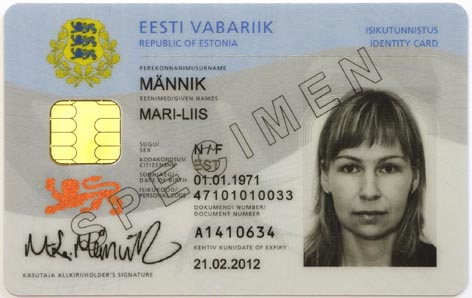
\includegraphics{idcard}

Вже у 2005 році вперше була випробована на реальному голосуванні система електронних виборів.
Вона була визнана успішною. 
Естонія стала першою країною світу, де стало можливим проголосувати через Інтернет. 

\subsection{Вимоги до електронного голосування}
Задля того, щоб побудувати систему електронного голосування, спочатку треба визначитися з вимогами, які
ця система повинна задовольняти:


\begin{enumerate}
    \item голосувати може лише зареєстрована людина;
    \item кожен може проголосувати лише один раз;
    \item усі голоса враховуються анонімно: зберігається таємниця виборів;
    \item проголосувавши, ми не маємо змоги змінити своє рішення;
    \item неможливість підробки результатів голосування;
    \item повинна бути можливість відкрито перевірити результати голосування;
    \item ми повинні мати змогу взнати, скільки людей проголосувало.
\end{enumerate}

Як ми бачимо, виставленні вимоги до системи, десь співпадають, а десь перевищують можливості звичайного
голосування. Проте давайте розглянемо, як усю цю купу вимог реалізувати на практиці.

\subsection{Схема електронного голосування}

Зазвичай організацією виборів займається якась державна структура.
В електронному голосуванні також маємо структуру, яка відповідає за організацію 
виборів. Назвемо її виборчим центром $\Sigma$.

В нашого виборчого центру, як і в кожного чемного виборчого центру існує довірена
особа $D$, яка буде виконувати функції обробки голосів виборців.

Самих виборців позначимо $A_i, i=\overline{1,N}$. Звісно, що в кожного виборця є
якась своя унікальна комбінація параметрів $D_i$, яка його ідентифікує. 
Також, у кожного виборця є своя RSA пара відкритого ключа $(n_i,e_i)$ і 
секретного ключа $d_i, i=\overline{1,N}$.

Перед початком самих виборів ми повинні скласти список усіх учасників процесу.
Зазвичай, цим займається виборчий центр. Виходячи з тієї інформації, що в нас є
логічно зберігати список виборців у вигляді:

\[ T = \left \{ <D_i, (n_i,e_i), i = \overline{1,N} \right\} \]

У довіреного лиця також є своя RSA із відкритим ключем $(m,e)$ і таємним ключем $d$.

\subsection{Процедура голосування виборців}

Нехай в нас існує $r$ можливих варіантів, за кого голосувати. $r-1$ кандидат і один варіант "Проти всіх".

Розглянемо приклад, коли в нас є наступні кандитати:

\begin{enumerate}
    \item Фідель
    \item Мао
    \item Наполеон
    \item Нельсон
\end{enumerate}

Спочатку, виборчий центр обирає кодування для кандидатів. Візьмемо варіант, коли $i-ий$ кандидат
представлен $i-им$ простим числом. Тобто для нашого варіанту маємо:

\begin{itemize}
    \item Фідель 2
    \item Мао 3
    \item Наполеон 5
    \item Нельсон 7
    \item Проти всіх 1
\end{itemize}

І ось настає славетна година, коли виборець $A_i$ йде на вибори -
до компьютера голосувати за свого кандидата $b_i$. 

Спочатку він, як і кожен чемний виборець, сгенерує своє просте число $q_i$, котре більше за 
усі числа-коди кандидатів. (У нашому прикладі $q_i>7$)

Обчислює $t_i=b_i*q_i$ за умови, що $b_i*q_i<m$, де $m$ - це частина відкритого ключа для $D$.

Після цього він зашифровує свій власний вибір $t_i$ відкритим ключем довіреного лиця $D$
\[ C_i = (t_i)^e mod\ m \].

Коли задача конфіденційності вирішена, потрібно ще вирішити задачу цілісності, тому ми підписуємо 
нашу "бюлетень" цифровим підписом:

\[ S_i = (h(D_i || C_i))^{d_i} mod \ m \] 
де $i = \overline{1,N}$, а h(.) - геш-функція

І тільки після цього ми передаємо свій зашифрований бюлетень виборчому центру:

\[ M_i = (D_i,\ C_i,\ S_i) \rightarrow \Sigma\]  

Після того, як усі охочі виборці зроблять свій вибір, вибори закриваються, і ми переходимо до етапу 
підрахунку голосів.

\subsection{Підрахунок голосів Sigm-ою}

Спочатку, довірча особа $D$ перевіряє цифровий підпис кожного виборця $A_i, i=\overline{1,N'}$:
\begin{enumerate}
    \item Спочатку йде перевірка, чи була особа $D_i$ зареєстрована для участі у виборах.
    \item Потім перевіряємо валідність цифрового підпису: 
    \[h(D_i||C_i)^{e_i}\ mod\ n_i\ ?=?\ h(D_i, C_i) \]
    
    \item Далі, якщо усі перевірки до цього пройдені, то $D$ розшифровує повідомлення:
    \[ {t_i}^d\ mod\ n = b_i\ *\ q_i\]
    та помічаємо $A_i$, як проголосувавшого.

    \item Останнім кроком $D$ вираховує значення:
    \[ Q = \prod_{i=1}^N \ b_i\ *\ q_i\]

    та відправляє його до виборчого центру $\Sigma$.
\end{enumerate}

Виборчий центр розкладує $Q$ на множники 
\[ Q = 2^{r_1}\ *\ 3^{r_2}\ *\ 5^{r_3}\ *\ 7^{r_4}\ *\ R\]
де $R = \prod_{i=1}^{N'}\ q_i$

І саме з розкладу визначає розподіл голосів по кандидатах.

Після підрахунку результати публікуються у формі:
\[ \{\ \{<D_i,C_i>, i=\overline{1,N'}\}\ ,\ r_1,\ r_2, ...\ ,\ r_k,\ N-\sum_{i=1}^{N'}r_i ,\ R,\ N-N' \} \]

де $N-\sum_{i=1}^{N'}r_i$ - це кількість голосів відданих варіанту "Проти всіх";

$N-N'$ - це кулькість не голосувавших виборців.

\subsection{Перевірка результатів голосування}

\begin{enumerate}
    \item Кожен виборець має змогу впевнетися, що його голос був зарахований по таблиці результатів.
    Тобто, воно буде присутнє в опублікованих даних виборів.

    Якщо ж виборець не голосував, то він не знайде себе серед опублікованих зашифрованих повідомлень.
    
    \item Таємниця голосування забезпечується для усіх, окрім довіреного лиця $D$.

    \item Як ми можемо бачити із схеми голосування, проголосувати за когось іншого неможливо. Підробити
    голос також.

    \item Перевірку правильності підрахунку голосів може перевірити будь-яка людина.

    Перш за все, ми перевіряємо те, щоб $R$ не повинно ділитися на 2, 3, 5, 7 

    З результатів виборів легко відновлюється число $Q$. Задля того, щоб перевірити правильність
    результатів, усе, що нам потрібно - це впевнетися, що має місце такая рівність:
    \[ Q^e \ mod \ m = (\prod_{i=1}^{N'} C_i) \ mod \ m\]

    Дійсно, якщо усе вірно, то:
    \[ Q^e \ mod \ m = (\prod_{i=1}^{N'} 2^{r_1} * 3^{r_2} * .. * 7 ^{r_4} * \prod_{i=1}^N q_i)^e 
    \ mod \ m  = \prod_{i=1}^N (b_i*q_i)^e\ mod\ m = (\prod_{i=1}^{N'} C_i) \ mod \ m\]

\end{enumerate}